\section{Opis struktury projektu}

\subsection{Architektura systemu}
System został zbudowany w oparciu o wzorzec MVC (Model-Widok-Kontroler):
\begin{itemize}
    \item \textbf{Model}: Baza danych SQLite, klasy dziedziny takie jak Lot, Rezerwacja, Pasażer, Użytkownik.
    \item \textbf{Widok}: Interfejs użytkownika zrealizowany w Swing, z odpowiednimi formularzami do przeglądania dostępnych lotów, rezerwacji oraz zarządzania kontem użytkownika.
    \item \textbf{Kontroler}: Logika biznesowa aplikacji, odpowiedzialna za obsługę rezerwacji, płatności oraz interakcje z bazą danych.
\end{itemize}

\subsection{Diagram klas}
\begin{figure}[H]
\centering
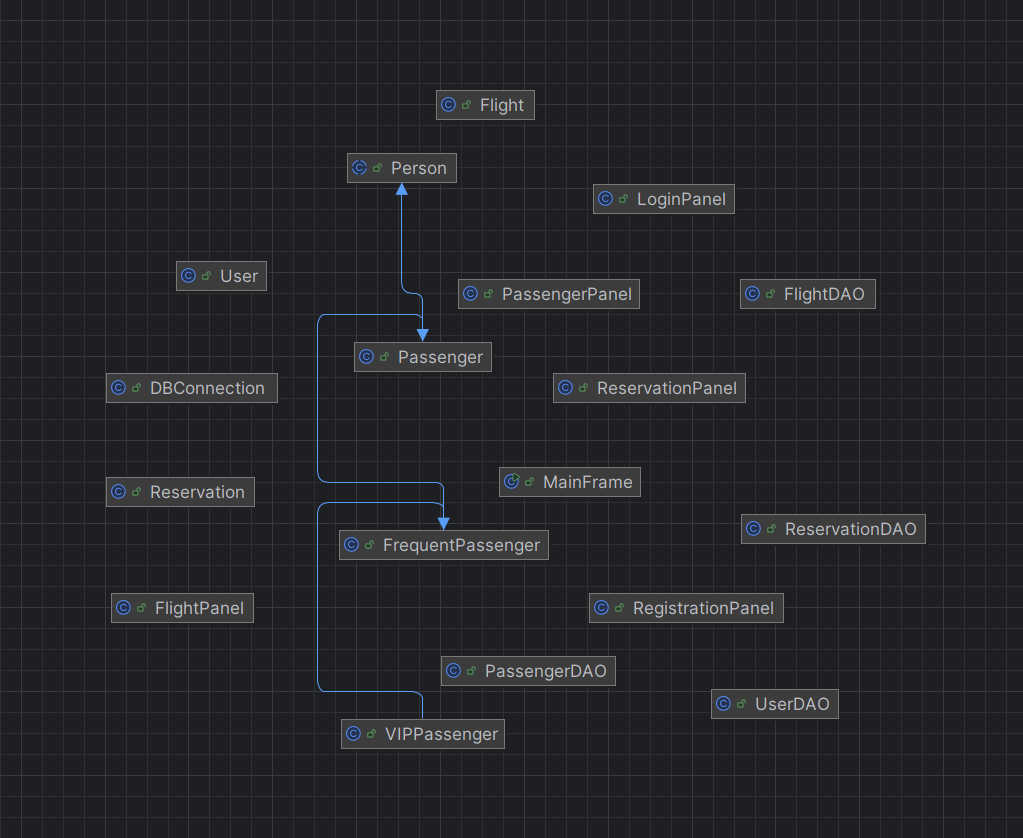
\includegraphics[width=0.9\textwidth]{figures/class_diagram.png}
\caption{Diagram głównych klas systemu}
\label{fig:class_diagram}
\end{figure}

Kluczowe klasy systemu:
\begin{itemize}
    \item \textbf{MainFrame}: Główne okno aplikacji, które uruchamia interfejs użytkownika i umożliwia interakcję z systemem.
    \item \textbf{Flight}: Klasa reprezentująca dane o locie, takie jak numer lotu, miejsce początkowe, miejsce docelowe oraz godziny odlotu i przylotu.
    \item \textbf{Passenger}: Klasa reprezentująca dane pasażera, takie jak imię, nazwisko, numer paszportu oraz historia rezerwacji.
    \item \textbf{Reservation}: Klasa odpowiadająca za dane o rezerwacji, powiązana z pasażerem oraz lotem.
    \item \textbf{User}: Klasa reprezentująca użytkownika aplikacji (dane logowania, poziom uprawnień).
    \item \textbf{DatabaseManager}: Klasa odpowiedzialna za dostęp do bazy danych i wykonywanie operacji na tabelach.
\end{itemize}

\subsection{Baza danych}
System wykorzystuje bazę danych SQLite, w której przechowywane są dane o lotach, rezerwacjach, pasażerach i użytkownikach. Baza danych składa się z następujących tabel:



\begin{figure}[H]
\centering
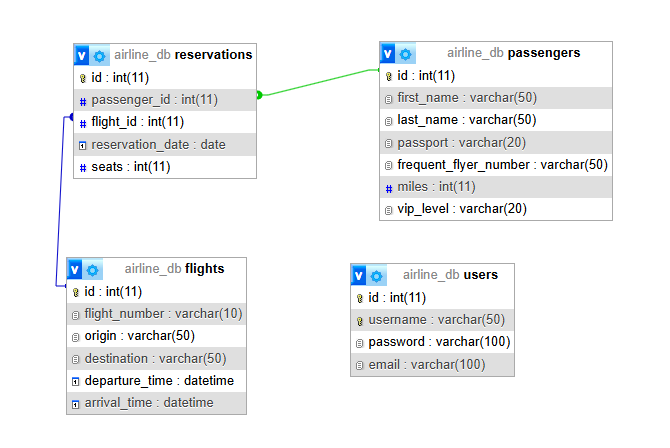
\includegraphics[width=0.8\textwidth]{figures/ERD_diagram.png}
\caption{Diagram ERD bazy danych}
\label{fig:erd_diagram}
\end{figure}
